\section{Experimental Setup}

\subsection{Experimental Settings}
All experiments were conducted on a dedicated server equipped with an \textit{NVIDIA RTX 4500 Ada Generation GPU} with \textit{24 GB} of VRAM, running CUDA version 12.5 and driver version \textit{555.42.06}. The system further consisted of a multi-core Intel CPU and 64 GB of RAM, running Ubuntu Linux (64-bit). Our implementation is based on Python 3.10 with \texttt{scikit-learn} and \texttt{xgboost} for learning-to-rank, and HuggingFace \texttt{transformers} for optional CodeBERT embeddings. To ensure reliable evaluation, we adopted a 5-fold stratified cross-validation strategy~\cite{stone1974cross}. For each repository, the labeled data was divided into five folds, with four folds used for training and the remaining fold reserved for testing. All reported results represent the average performance across the five folds, providing a balanced and consistent protocol for assessing model effectiveness across projects.


% Training and inference were executed in mixed-precision mode where applicable to maximize efficiency. Unless otherwise specified, all reported results are averaged over three independent runs with identical hyperparameters to account for variance.





% \subsection{Evaluation Metrics}


% In a one-to-many relationship, an issue may be associated with multiple commits. Therefore, evaluating each issue-commit pair independently does not reflect the model's effectiveness in recovering complete commit sets for issues. To address this, we adopt an issue-wise evaluation strategy, where each \textit{Issue\_ID} (represents an issue with a set of commits) is treated as a unit. For every issue, we compute the confusion matrix components, True Positives ($TP$), False Positives ($FP$), False Negatives ($FN$), and True Negatives ($TN$), based on the set of predicted and actual linked commits. These values are then used to calculate Precision, Recall, and F1-score per issue. Finally, we report the average of these scores across all issues to provide an overall measure of model performance.

% \paragraph{Precision ($Precision_{one-to-many}$)}

% Precision in the one-to-many setting measures the proportion of correctly predicted commits among all commits predicted to be linked to an issue.

% \[
% \text{Precision}_{\text{one-to-many}}^{(i)} = \frac{TP_i}{TP_i + FP_i}
% \]

% Where:
% \begin{itemize}
%     \item $TP_i$: Number of true positives for issue $i$ (correctly predicted linked commits).
%     \item $FP_i$: Number of false positives for issue $i$ (commits incorrectly predicted as linked).
% \end{itemize}

% The overall precision is computed as the average across all issues:
% \[
% \text{Precision}_{\text{one-to-many}} = \frac{1}{|I|} \sum_{i \in I} \text{Precision}_{\text{one-to-many}}^{(i)}
% \]

% \paragraph{Recall ($Recall_{one-to-many}$)}

% Recall measures the ability of the model to retrieve all relevant commits for an issue.

% \[
% \text{Recall}_{\text{one-to-many}}^{(i)} = \frac{TP_i}{TP_i + FN_i}
% \]

% Where:
% \begin{itemize}
%     \item $FN_i$: Number of false negatives for issue $i$ (linked commits not predicted).
% \end{itemize}

% The average recall across all issues is:
% \[
% \text{Recall}_{\text{one-to-many}} = \frac{1}{|I|} \sum_{i \in I} \text{Recall}_{\text{one-to-many}}^{(i)}
% \]

% \paragraph{F1-Score ($F1_{one-to-many}$)}

% The F1-score balances precision and recall for each issue:

% \[
% \text{F1}_{\text{one-to-many}}^{(i)} = \frac{2 \cdot \text{Precision}^{(i)} \cdot \text{Recall}^{(i)}}{\text{Precision}^{(i)} + \text{Recall}^{(i)}}
% \]

% And the final F1-score is computed by averaging:
% \[
% \text{F1}_{\text{one-to-many}} = \frac{1}{|I|} \sum_{i \in I} \text{F1}_{\text{one-to-many}}^{(i)}
% \]

\subsection{Evaluation Metrics}

In a one-to-many relationship, an issue may be linked to multiple commits. Evaluating each issue--commit pair independently fails to capture how effectively a model recovers the complete set of commits for an issue. To address this, we adopt an \emph{issue-wise evaluation} strategy: each issue $i$ (identified by its \textit{Issue\_ID}) is treated as a single evaluation unit. For every issue, we compute the confusion matrix components—True Positives ($TP_i$), False Positives ($FP_i$), and False Negatives ($FN_i$)—from which we derive Precision, Recall, and F1-score. The final results are obtained via \emph{macro-averaging}, ensuring that all issues contribute equally regardless of their number of linked commits.

\paragraph{Precision and Recall.}
Precision quantifies correctness, while Recall measures completeness of retrieved commits for each issue:
\[
\text{Precision}^{(i)} = \frac{TP_i}{TP_i + FP_i}, \qquad
\text{Recall}^{(i)} = \frac{TP_i}{TP_i + FN_i}.
\]
The overall scores are macro-averaged across all issues:
\[
\text{Precision} = \frac{1}{|I|}\sum_{i \in I}\text{Precision}^{(i)}, \qquad
\text{Recall} = \frac{1}{|I|}\sum_{i \in I}\text{Recall}^{(i)}.
\]

\paragraph{General F$_\beta$-Score.}
The F$_\beta$-score provides a weighted harmonic mean of Precision and Recall, allowing control over their relative importance through the parameter $\beta$:
\[
\text{F}_{\beta}^{(i)} = (1+\beta^2)\frac{\text{Precision}^{(i)} \cdot \text{Recall}^{(i)}}{(\beta^2 \cdot \text{Precision}^{(i)}) + \text{Recall}^{(i)}}.
\]

\paragraph{F1-Score and Its Choice.}
For $\beta = 1$, the F$_1$-score simplifies to:
\[
\text{F1}^{(i)} = \frac{2 \cdot \text{Precision}^{(i)} \cdot \text{Recall}^{(i)}}{\text{Precision}^{(i)} + \text{Recall}^{(i)}}, \qquad
\text{F1} = \frac{1}{|I|}\sum_{i \in I}\text{F1}^{(i)}.
\]

We choose the F1-score because it provides a balanced measure of performance when both false positives (over-linking commits to an issue) and false negatives (missing true links) are equally important. In the issue--commit linking context, over-predicting leads to noisy traceability, while under-predicting omits valid relationships—thus, F1 offers a fair trade-off between precision and recall, capturing the model’s overall linkage accuracy.



% \paragraph{Jaccard Similarity.}
% In addition to precision, recall, and F-score, we also evaluate performance using the Jaccard coefficient, which provides a stricter measure of set-level similarity. For each issue $i$, let $C(i)$ denote the set of ground-truth linked commits and $\widehat{C}(i)$ the set of predicted commits. The Jaccard index is defined as:
% \[
% J(i) = \frac{|C(i) \cap \widehat{C}(i)|}{|C(i) \cup \widehat{C}(i)|}.
% \]

% Unlike pairwise metrics that consider links independently, Jaccard directly measures the overlap between the predicted and actual commit sets. This makes it particularly suitable for one-to-many linking, where recovering the complete set of commits associated with an issue is essential. For example, if an issue is linked to four commits and the model predicts three of them correctly but adds one incorrect commit, precision and recall may appear high, but the Jaccard score will penalize the discrepancy by considering the entire set overlap.  \\

% \noindent
% By averaging $J(i)$ across all issues, we obtain a macro-level Jaccard score that reflects how well the model captures issue–commit sets in their entirety. This provides complementary insights beyond conventional precision and recall, highlighting the framework’s ability to achieve holistic traceability rather than partial correctness.


\subsection{Training and Inference Costs}

We conducted a comparative analysis of training and testing times across our approaches and the baseline models to answer the question:
\emph{How do LinkRank and LinkRank-C2I perform in terms of computational efficiency compared to existing baselines while maintaining high predictive accuracy?}\\

Figure~\ref{fig:time} presents efficiency (x-axis, in minutes, log scale) together with effectiveness (y-axis, F-score). Each line connects test (left dot) and train (right dot) times, while the y-axis annotates the corresponding F-scores. This visualization highlights the balance between computational cost and predictive performance. The results show that our LinkRank variants achieve strong predictive performance while remaining significantly more lightweight. For instance, LinkRank and LinkRank-C2I complete training within 30--40 minutes and testing within 5--7 minutes, yet yield F-scores above 83. In contrast, baselines such as DeepLink and EALink consume far more computational resources (160--225 minutes of training and 10--15 minutes of inference) while producing substantially lower accuracy.\\

\begin{figure}[htbp]
	\centering
	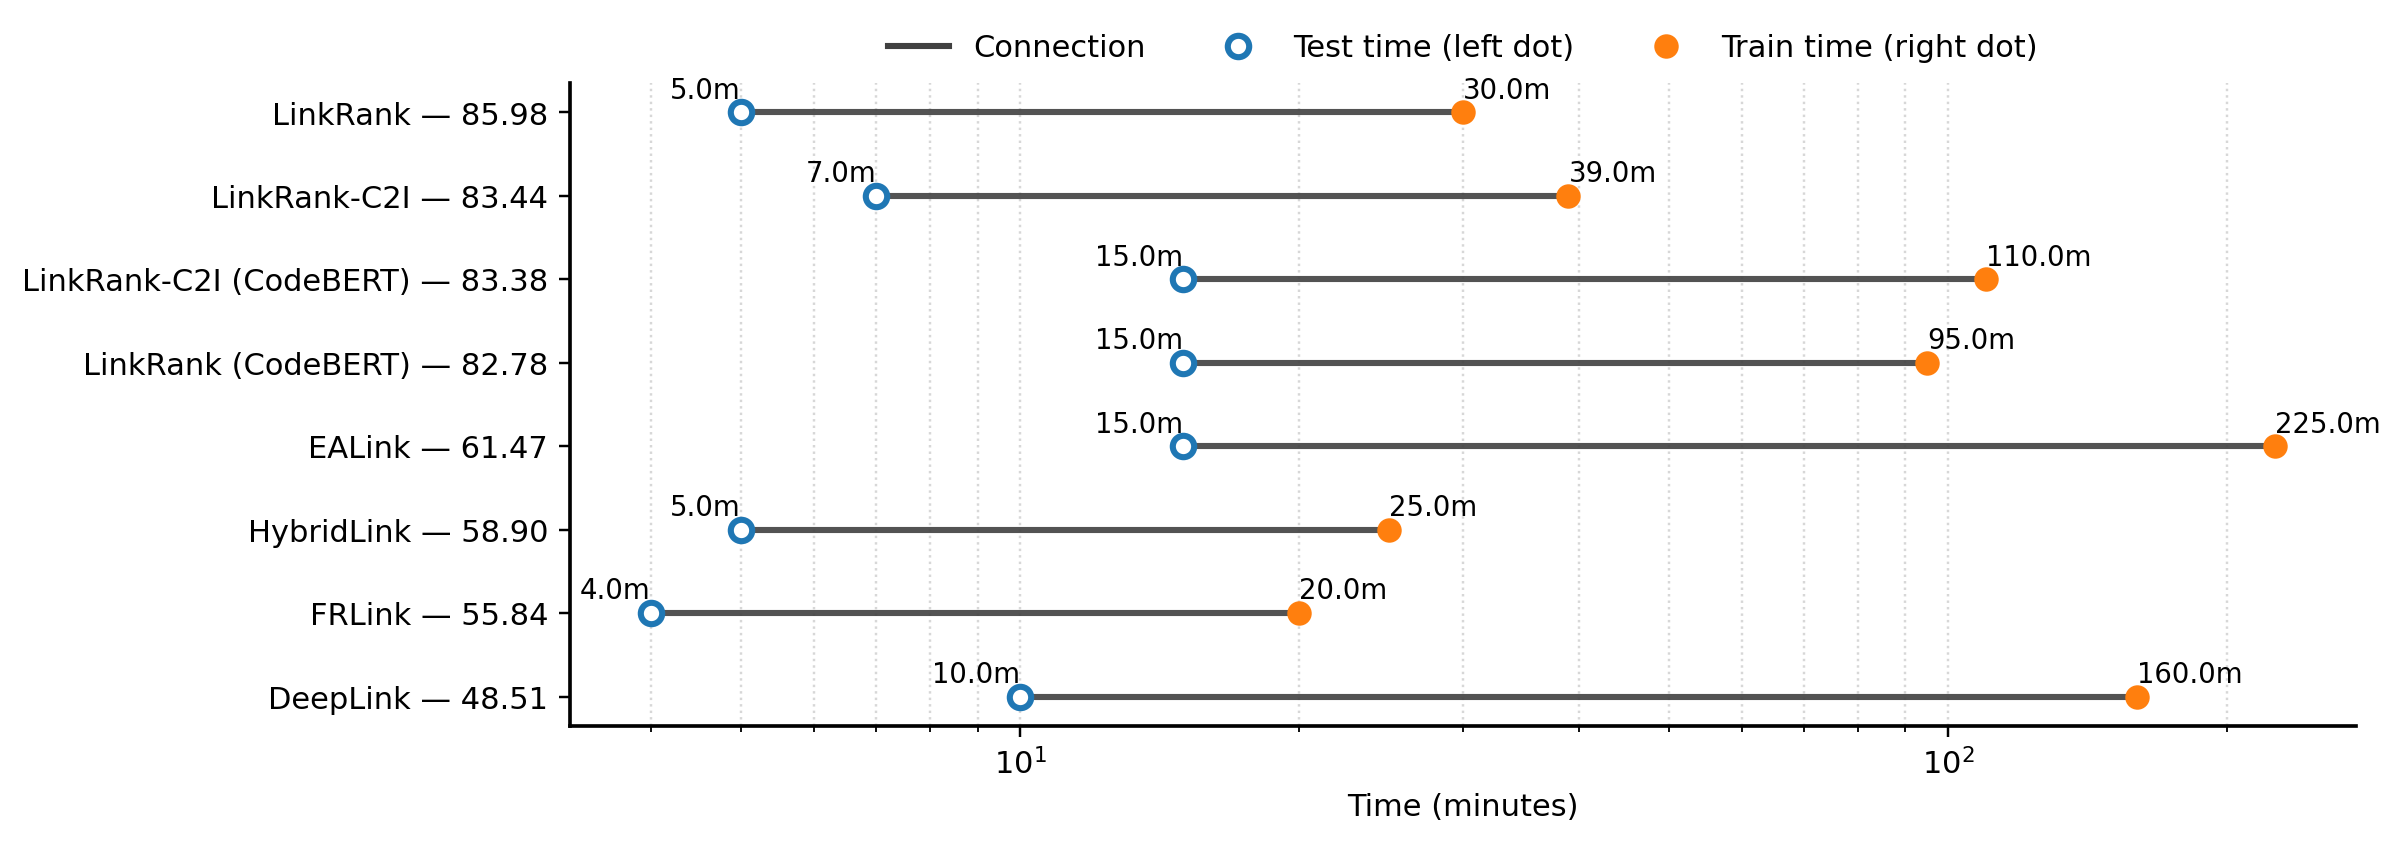
\includegraphics[width=\linewidth]{Figures/time.png}
	\caption{Training and inference time comparison of LinkRank, LinkRank-C2I, and baselines. }
	\label{fig:time}
\end{figure}

A key observation is that adding CodeBERT embeddings increases both training and testing costs by $3$--$4\times$ (e.g., 95--110 minutes of training), but delivers only marginal improvements in F-score. This highlights that the core design of LinkRank is already well suited for the largely pattern-matching nature of issue--commit recovery.




